\section{Coupler}

\begin{frame}[fragile,containsverbatim]\frametitle{PFLOTRAN Coupler}

\begin{itemize}
\item[] \textbf{Purpose:} Couples a flow and/or transport conditions with a region to create a boundary condition, initial condition or source/sink.
\item[] \textbf{Example uses:}
\begin{itemize}
  \item Assign a boundary condition to a face of the model
  \item Assign initial concentrations to a zone in the model
  \item Assign an injection well with in the model domain
\end{itemize}
\end{itemize}
\end{frame}

\begin{frame}[fragile,containsverbatim]\frametitle{PFLOTRAN Coupler}
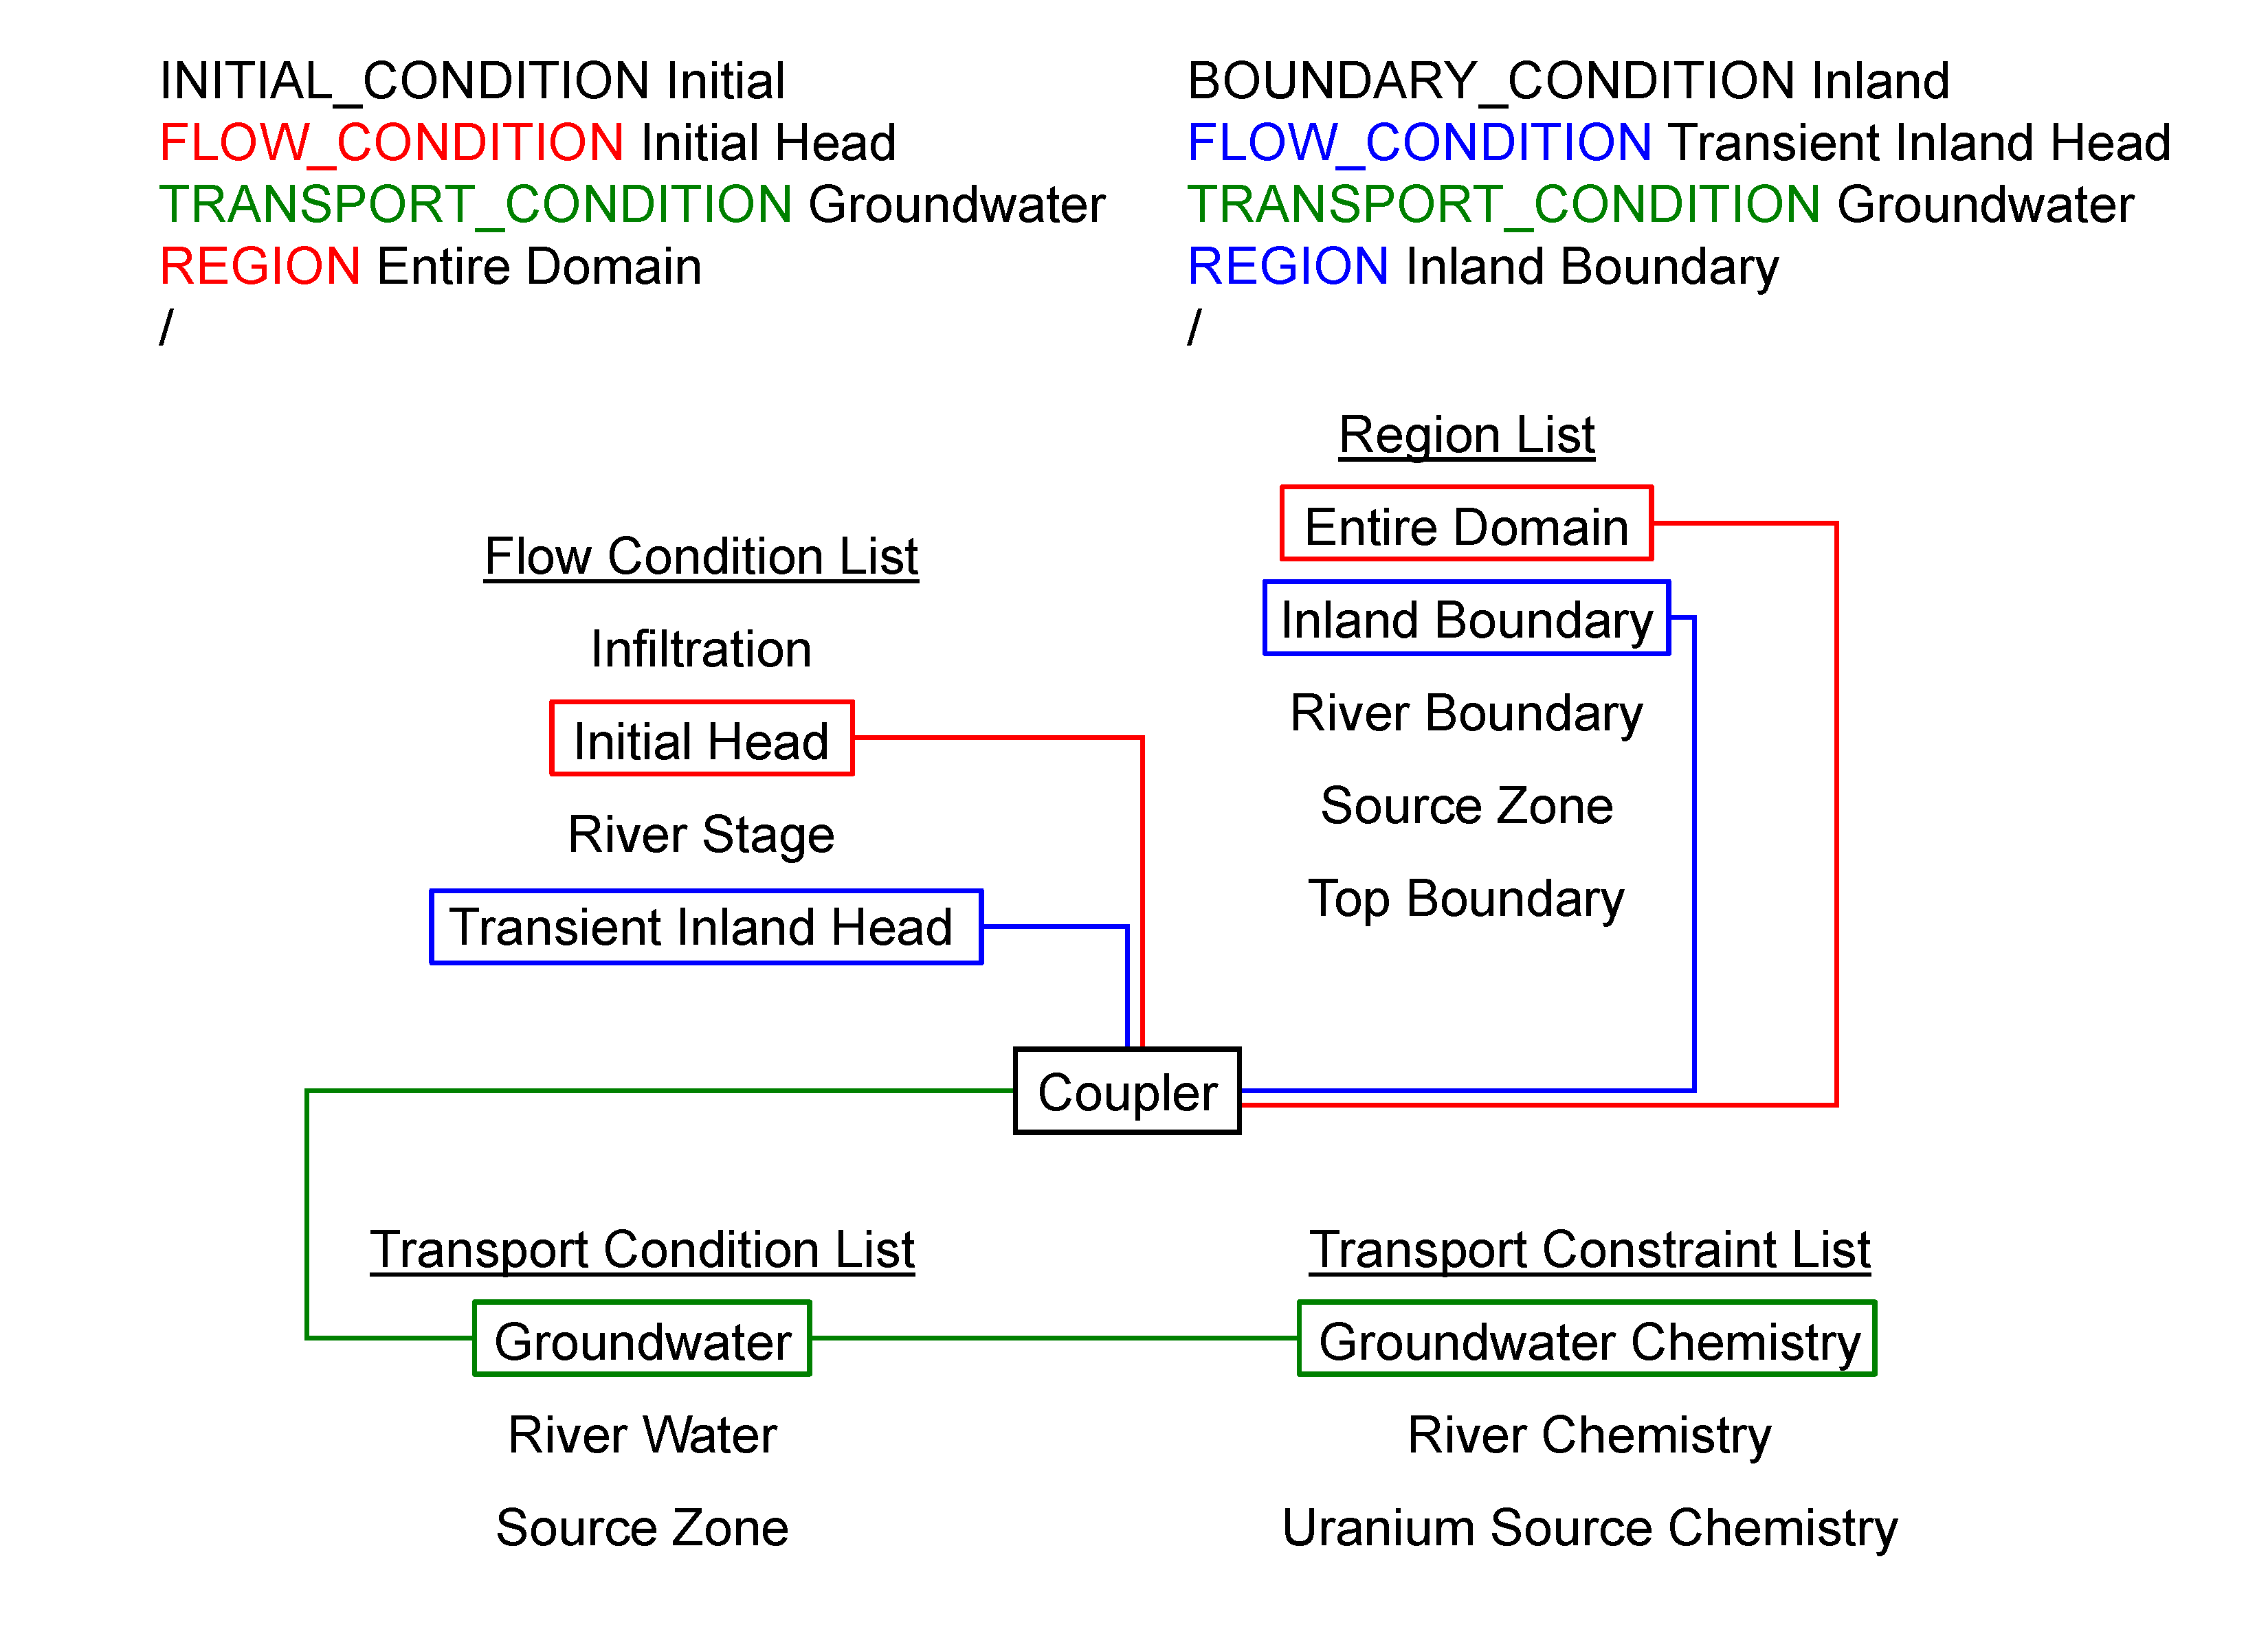
\includegraphics[width=\linewidth]{coupler.pdf}
\end{frame}
